\section{Additional Kernel Studies}
\label{app:kernel-studies}

This appendix is reserved for non-baseline kernel robustness studies. The production
workflow documented in the main text uses the single Constant$\times$RBF model of
Section~\ref{sec:kernel-choice}; alternative kernels are treated only as cross-checks,
not as competing headline methods.

The first comparison to be frozen here will be a Constant$\times$Mat\'ern$(\nu=3/2)$
study with the same resolution-scaled length-scale bounds used by the baseline model.
That choice isolates one physically relevant assumption, namely the degree of smoothness
allowed in the continuum background, without changing the overall stationary
smooth-background prior class.

When the comparison suite is finalized, this appendix will summarize the resulting
shifts in blind-window mean and covariance, fitted signal yield, pull mean and width,
coverage, and expected $\eps^2$ limits relative to the production RBF baseline.
Earlier piecewise-window variants and wider/narrower length-scale-bound studies will
also be collected here once their note-quality exports are frozen.
\subsection{Uncertainty Propagation}

The total uncertainty $\sigma_{total}$ is calculated as

$\sigma_{total} = \sqrt{\sigma_{model} + \sigma_{n}}$

where $\sigma_{model}$ is the predictive variance of the GP and $\sigma_n$ is the Poisson statistical uncertainty, typically modeled in our studies with a WhiteKernel. The predictive variance of the GP is found
$\sigma_{model}^2(x_*) = k(x_*, x_*) - k_*^T \left( K + \sigma_n^2 I \right)^{-1} k_*$
where K is the covariance between training points, $k_*$ is the covariance between a test point and training points. $k(x_*,x_*)$ is the prior variance of the GP at $x_*$.

\subsection{Kernels Definition}
All kernels used in these studies will be defined in this section.
\subsubsection{Radial Basis Function (RBF)}
$k(x_i, x_j) = \exp\left(-\frac{d(x_i, x_j)^2}{2l^2}\right)$


The RBF kernel is defined by a length scale parameter $l$ and Euclidian distance $d(.,.)$ between measurements $x_i$ and $x_j$. Because it is infinitely differentiable, the RBF kernel models smoothness, and thus is very useful in GPR of mass distributions.
\subsubsection{Matern}
$C_{\nu}(d) = \sigma^2 \frac{2^{1-\nu}}{\Gamma(\nu)} \left( \sqrt{2\nu} \frac{d}{\rho} \right)^{\nu} K_{\nu}\left( \sqrt{2\nu} \frac{d}{\rho} \right)$


The Matern kernel defines the covariance between two measurements using the distance $\nu$ between them. $\Gamma$ is the Gamma function and $K_\nu$ is a modified Bessel function of the second kind.

$K_{\nu}(x) = \frac{1}{2} \int_{0}^{\infty} t^{\nu - 1} \exp\left(-\frac{x}{2}\left(t + \frac{1}{t}\right)\right) , dt$

\subsubsection{WhiteKernel}
$k(x_i, x_j) = noise\_level$ if $x_i == x_j$ else 0

WhiteKernel captures the normally-distributed variance or noise of a signal. It takes one parameter $noise\_level$ which controls the variance of the kernel. 

\subsubsection{DotProduct}
$k(x_i, x_j) = \sigma_0^2 + x_i + x_j$

The DotProduct parameter $\sigma_0$ is set to zero for these studies, resulting in a homogeneous linear kernel, used to model linear components in distributions.

\subsection{Initial Global Fitting of 2016 Datasets}

Initial studies were global fits, in which a single GPR model was trained over the entire dataset. A combination of kernels was used. The original kernel consisted of an RBF kernel, multiplied by a linear kernel, with an added WhiteNoise kernel. This was meant to capture the linear trend in the dataset due to detector mass resolution while accounting for statistical uncertainty.

\begin{figure}
    \centering
    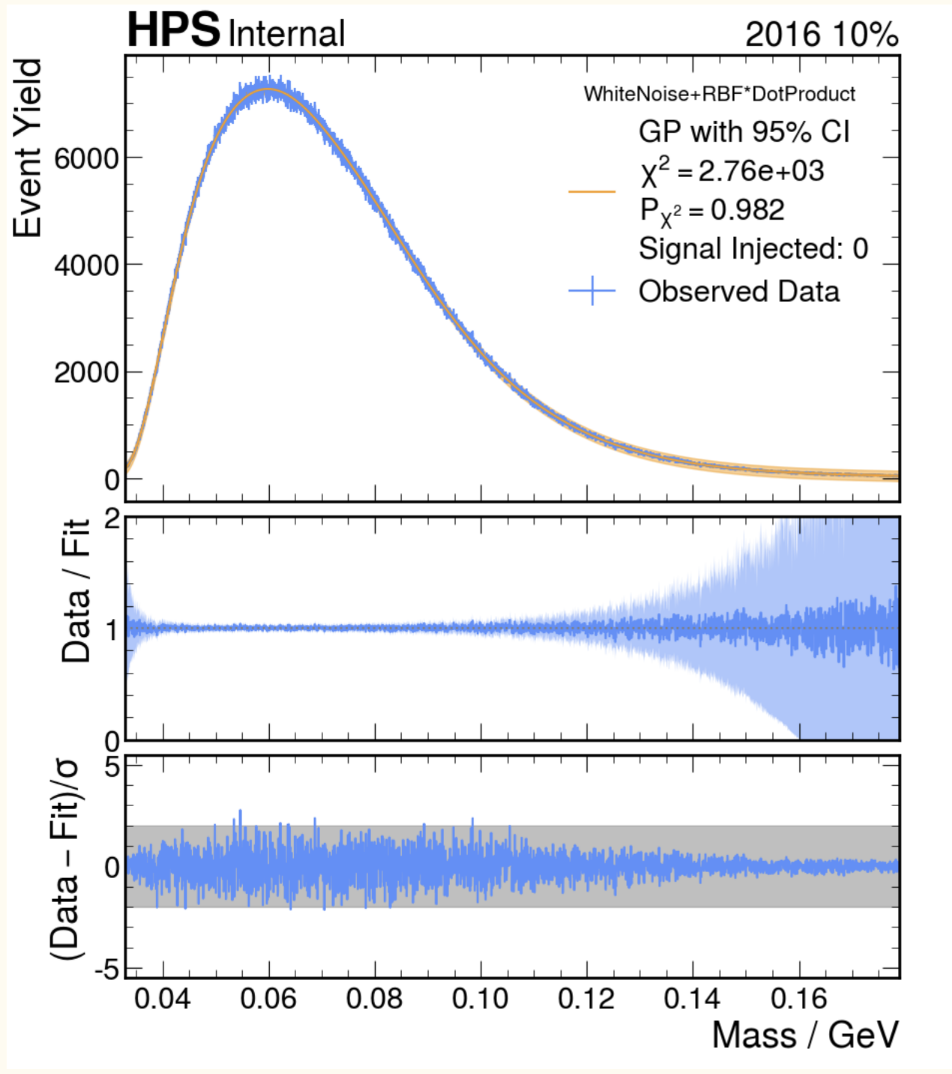
\includegraphics[width=0.86\linewidth]{appendix_figs/2016_10pct_whitenoisefit.png}
    \caption{Fit with a kernel consisting of a RBF kernel, multiplied by a linear kernel, with an added WhiteNoise kernel on the 2016 10\% dataset, with standardized residual.}
    \label{fig:appendix-whitenoisefit-2016}
\end{figure}

This global model represented an acceptable fit of the mass distribution, but lent itself to instability during applications in setting upper limits and calculating p-values.

\subsection{Piecewise Fitting and Kernel "Softmax"}

A piecewise approach was introduced due to the unreliability of global fitting. In this method, the data was separated into sections surrounding a mass hypothesis mA'. Each section, with an A' at its center, would be fit by a distinct GP model, trained on the outer region while being blinded to the smaller inner section (not receiving the data inside as information during training).

\begin{figure}
    \centering
    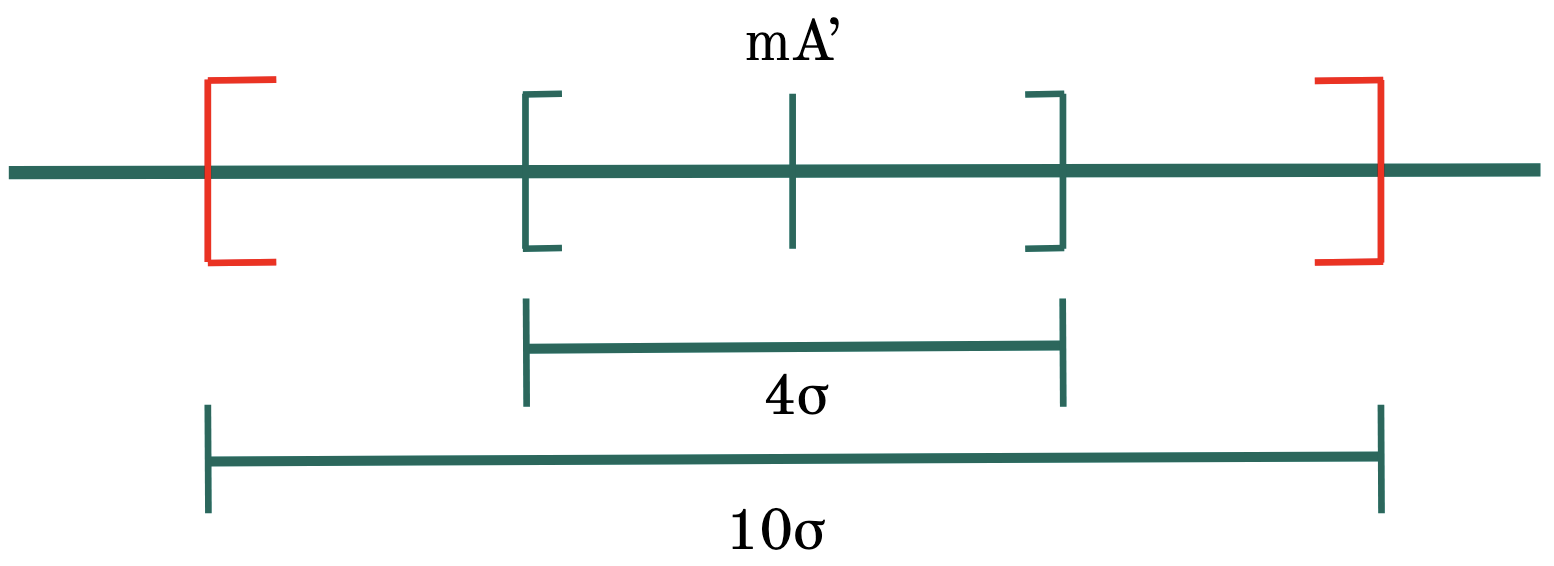
\includegraphics[scale=0.5]{appendix_figs/piecewise_diagram.png}
    \caption{A schematic of a section surrounding an mA'. The training region had a total width of 10$\sigma$, where $\sigma$ is the mass resolution. The inner blinded region had a width of 5$\sigma$. The GPR models did not have information about their sections' blinded regions and interpolated the region.}
    \label{fig:appendix-piecewise-diagram}
\end{figure}

The kernel used by each section's model was selected from an ensemble using a procedure that chose the best performing kernel. For each section, every kernel as a part of the kernel ensemble was tested in an interpolation of the blinded region. Each kernel was given a score by log marginal likelihood, and this vector of scores was converted to weights via a softmax function. A kernel would be sampled from the distribution of these weights and used by a GP to determine the distribution of the blinded region. Poisson observed counts are sampled using this chosen distribution.
\begin{figure}[h!]
    \centering
    $w_k = \frac{e^{\ell_k - \max_j \ell_j}}{\sum_j e^{\ell_j - \max_j \ell_j}}$
    $\quad \text{with} \quad$
    $\ell_k = \log p(\text{data} \mid K_k).$
    \caption{the softmax function used to convert the log marginal likelihood of each kernel to a weight.}
    \label{fig:appendix-softmax}
\end{figure}

\subsection{Piecewise Upper Limits}

Upper limits on the signal yield and coupling strength $\epsilon^2$ were measured using this piecewise method. Values for the upper limit on the signal yield, or the maximum number of expected signal events, were calculated using
$s_{up} = \frac{1}{2}F^{-1}_{2(n+1)}(p) - b$
where b is the expected number of Poisson background, alpha = 0.05 for 95$\%$ confidence, F is the chi-squared cumulative distribution for 2(n+1) degrees of freedom, and $n$ is the observed number of events.


\begin{figure}
    \centering
    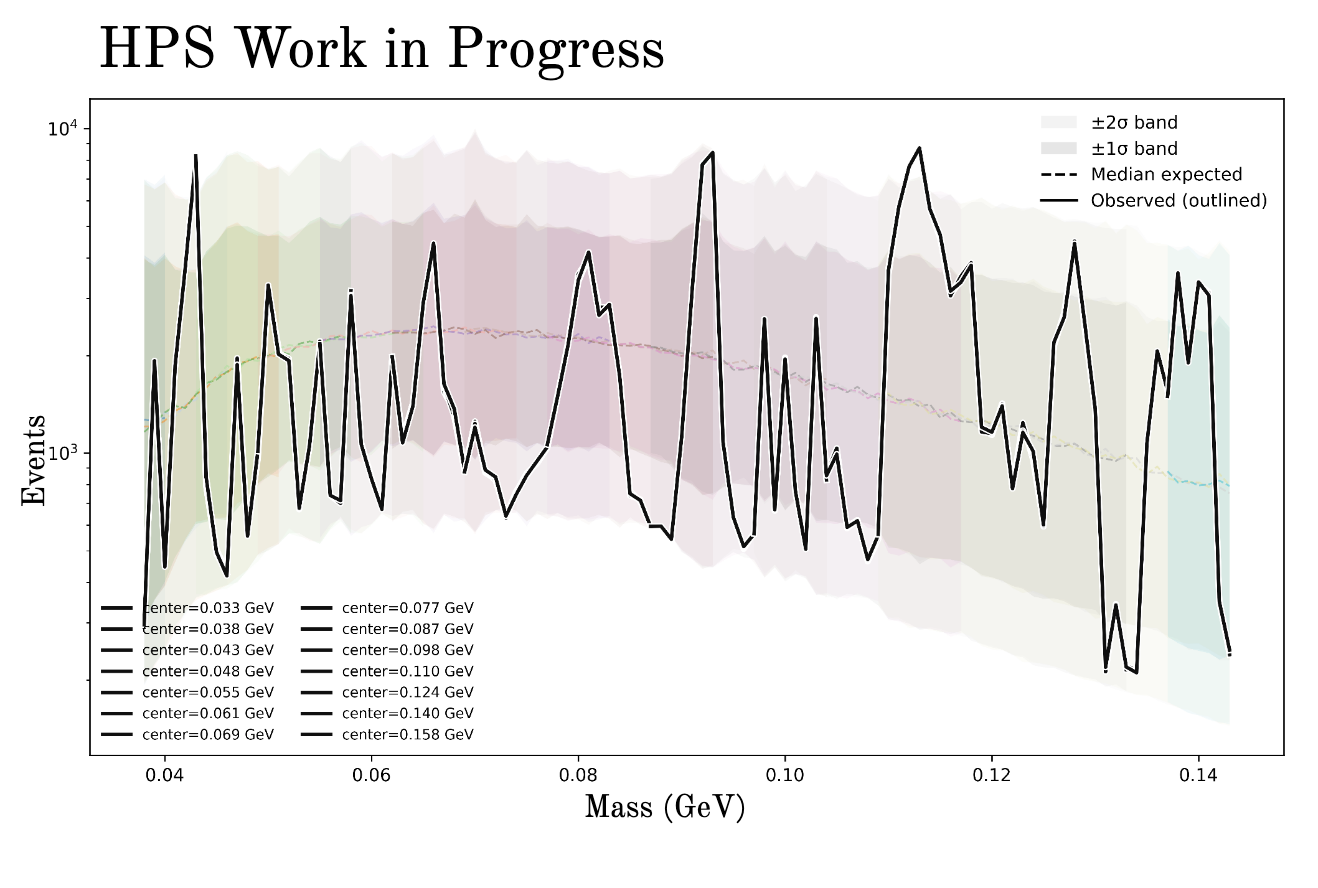
\includegraphics[scale=0.5]{appendix_figs/signal_yield_2016_10.png}
    \caption{The upper limit on the signal yield for the 2016 10\% dataset. The shade of the uncertainty bands reflect the size of each region.}
    \label{fig:appendix-signal-yield-2016}
\end{figure}

\subsection{Guard-Band Construction Reference}
\label{app:guard-band-construction}

The guard-band construction considered during the 2015 closure campaign separated each
mass hypothesis into three regions: a central blind/extraction window, an adjacent
guard band omitted from both training and extraction, and outer sidebands used to train
the GP. In the notation of the main text, the central blind region covered
$|m-m_0|<1.64\,\sigma_m$, while the guard excluded
$1.64<|m-m_0|/\sigma_m<2.25$ from the sideband training sample. This construction is
useful as a signal-leakage control diagnostic, but the refmatched geometry comparison in
Section~\ref{subsec:guard-band-construction} selects the $2.25\,\sigma_m$
blind/extraction window because it keeps the same training protection while retaining
the signal tails in the likelihood.

\begin{figure}[H]
\centering
\graphicorplaceholder{0.88\linewidth}{guard_band_figs/guard_band_signal_leakage_cartoon.png}
\caption{Reference cartoon for the older guard-band construction. The red central
region is the $1.64\,\sigma_m$ blind/extraction window, the yellow bands are excluded
from GP training as a guard, and the green sidebands train the background. This
construction motivated the training-exclusion study but is superseded in the main text
by the $2.25\,\sigma_m$ blind-window geometry.}
\label{fig:appendix-guard-band-cartoon}
\end{figure}
